%************************************************
\chapter{Grundlagen}\label{kap:grundlagen}
%************************************************
In diesem Kapitel werden die erforderlichen Grundlagen beschrieben, auf denen die Auslegung der Simulation, der Bewertung der Ergebnisse und die prototypische Implementierung aufbauen. Dabei gliedert sich das Kapitel in 5 Teile: \autoref{kap:grundlagen_sec:funk} und \autoref{kap:grundlagen_sec:protokolle} behandeln Grundzüge der Funkkommunikation sowie den damit verbunden Verarbeitungsvorschriften für die Systemsoftware, den Protokollen. Es folgt \autoref{kap:grundlagen_sec:energieverbrauch} mit relevanten Faktoren und Diagnosemöglichkeiten hinsichtlich des Energieverbrauchs bei Funkkommunikation. \autoref{kap:grundlagen_sec:simulation} gibt eine Einführung in ereignisorientierte Simulationen. In \autoref{kap:grundlagen_sec:hardware} werden die verwendeten Hardwareplattformen und ihre Besonderheiten vorgestellt.

\section{Funkkommunikation}\label{kap:grundlagen_sec:funk}

\begin{figure}[bth]
        \myfloatalign
        {\includegraphics[width=1\linewidth]{gfx/Spektrum}} 
        \caption[Spektrum]{Einordnung von Funkwellen im elektromagnetischen Spektrum}\label{fig:spektrum}
\end{figure}

Funkkommunikation ist die Übertragung von Informationen durch elektromagnetische Wellen. Dabei stehen Funkwellen verschiedener Frequenzen als Übertragungsmedium zu Verfügung. Abschnitte des Funkspektrums werden Bänder genannt. Ein Frequenzband kann je nach Anwendung in weitere Abschnitte, den sogenannten Kanälen, unterteilt werden. Der Radio- und Fernsehrundfunk, der Mobilfunk oder Satellitenübertragungen sind typische Beispiele. Aber auch \acs{wlan}, \gls{bluetooth}, schnurlose Telefone, Rauchmelder oder \acsp{wsn} nutzen Funkwellen zum Informationsaustausch. Eine Einordnung der Funkwellen im gesamten elektromagnetischen Spektrum ist in \autoref{fig:spektrum} zu sehen. Den verschiedenen Anwendungen sind dabei bestimmte Frequenzabschnitte zugeordnet.  Diese Zuordnung ist teilweise mit kostenpflichtigen Lizenzen versehen, die in Deutschland die Bundesnetzagentur verwaltet. So werden \zB einzelne Frequenzbereiche an Mobilfunkanbieter versteigert. Neben den lizensierten Bändern, stehen auch Bereiche speziell für den Einsatz in Industrie, Wissenschaft und Medizin zur Verfügung. Diese Frequenzen werden im \gls{ism} Band zusammengefasst. Die in Deutschland zur Verfügung stehenden Bereiche befinden sich u.a. im $434MHz$ Band, im $2,4GHz$ Band und im $5,7 GHz$ Band. Der $868MHz$ ist vornehmlich für Alarmfunkanlagen vorgesehen. Der Bereich $868,6MHz - 868,7MHz$ steht jedoch auch für allgemeinen Datenaustausch zur Verfügung \citep{ISMBand}.

\subsection{Freiraumausbreitung}\label{kap:grundlagen_sec:wellenausbreitung}

\begin{figure}[bth]
        \myfloatalign
        {\includegraphics[width=0.6\linewidth]{gfx/Funkausbreitung}} 
        \caption[Ausbreitung]{Idealisierte Funkwellenausbreitung mit isotropen Antennen}\label{fig:Isotropstrahler}
\end{figure}

Zur Beschreibung der Wellenausbreitung seien zunächst isotrope Strahler betrachtet, also Antennen, von denen sich die Funkwellen mit der Lichtgeschwindigkeit $c$ gleichmäßig in alle Raumrichtungen ausbreiten, wie in \autoref{fig:Isotropstrahler} skizziert. Wird ein zu übertragenes Signal mit der Leistung $P\textrm{S}$ in eine solche Sendeantenne eingespeist, so verteilt sich diese Leistung im Abstand $r$ auf die Fläche einer Kugel mit Radius $r$. Die Leistungsdichte an einem beliebigen Punkt im Umfeld des Senders beträgt:
\begin{equation}
{S = \frac{P_\textrm{S}}{A_\textrm{Kugel}} = \frac{P_S}{4{\pi}r^2}}
\label{eq:leistungsdichte}
\end{equation}
Um der elektromagnetischen Welle Leistung zu entnehmen, muss die Empfangsantenne im mathematischen Sinn eine Fläche besitzen, die von der Leistungsdichte durchsetzt wird. Diese wird Antennenwirkfläche $A_W$ genannt.
\begin{equation}
{P_E = S  \cdot A_W}
\label{eq:pe1}
\end{equation}
Die Antennenwirkfläche ist nicht die geometrische Fläche der Antenne, sondern ein frequenzabhängiger Wert. Bei einer isotropen Antenne ist die Antennenwirkfläche definiert zu:
\begin{equation}
{A_W = \frac{c^2}{4{\pi}f^2}}
\label{eq:aw}
\end{equation}
Nach Einsetzen von \autoref{eq:aw} und \autoref{eq:leistungsdichte} in \autoref{eq:pe1} ergibt sich die Empfangsleistung:
\begin{equation}
{P_E = \frac{P_S}{4{\pi}r^2} \cdot \frac{c^2}{4{\pi}f^2} = P_S \cdot \left(\frac{c}{4{\pi}rf}\right)^2}
\label{eq:pe2}
\end{equation}

\begin{table}
    \myfloatalign
  \begin{tabularx}{0.5\textwidth}{Xll} \toprule
    \tableheadline{Abstand} & \tableheadline{$P_E$} \\ \midrule
    $10m$ & $0,57mW$ \\
    $20m$ & $0,14mW$ \\
    $30m$ & $0,06mW$ \\
    \bottomrule
  \end{tabularx}
  \caption[Empfangsleistung]{Empfangsleistung bei Freiraumausbreitung und isotropen Rundstrahler mit der Sendeleistung $1Watt$ bei $100MHz$}  \label{tab:empfangsleistung}
\end{table}

In \autoref{tab:empfangsleistung} sind exemplarisch die Empfangsleistungen einer Übertragung bei $100Mhz$ und eine Sendeleistung von $1Watt$ eingetragen. Dabei wird ersichtlich, dass am Empfänger nur noch ein Bruchteil der ursprünglichen Signalleistung zur Verfügung steht.
Die Verringerung der Sendeleistung wird Dämpfung genannt und als logarithmisches Maß in Dezibel angegeben. Sie ist das Verhältnis von $P_S$ zu $P_E$. Nach \autoref{eq:pe2} ergibt sich die \emph{Freiraumdämpfung} $F$ zu:

\begin{equation}
{F = 10\lg \left(\frac{P_S}{P_E}\right) = 10\lg\left(\frac{4{\pi}rf}{c}\right)^2 }
\label{eq:freiraumdämpfung}
\end{equation}

In \autoref{fig:Isotropstrahler} ist die Freiraumdämpfung für drei verschiedene Frequenzen des \gls{ism}-Bands über die Entfernung zwischen Sender und Empfänger aufgetragen. Es ist gut zu erkennen, dass hohe Frequenzen stärker gedämpft werden als niedrige.

\begin{figure}[bth]
        \myfloatalign
        {\includegraphics[width=1\linewidth]{gfx/Freiraumdaempfung}} 
        \caption[Freiraumdämpfung]{Freiraumdämpfung bei verschiedene Frequenzen}\label{fig:Isotropstrahler}
\end{figure}

Bei realen Antennen entspricht die abgestrahlte Leistung auf Grund von \zB ohmschen Verlusten innerhalb der Antenne, nicht der eingespeisten Leistung. Dieser Verlustfaktor, also das Verhältnis von abgestrahlter zu eingespeister Leistung wird durch den Antennenwirkungsgrad $\eta$ ausgedrückt. 

In der Regel strahlen Antennen nicht gleichmäßig in alle Raumrichtungen, wie in \autoref{fig:Isotropstrahler}. Antennen können speziell so konzipiert werden, dass sie die abgestrahlte Leistung in bestimmten Richtungen bündeln. Es kann \zB in einigen Anwendungen sinnvoll sein, wenn die Sendeantenne weniger stark nach oben und nach unten strahlt, dafür umso mehr in die Breite. Das ist bei Dipolantennen der Fall. Ein weiteres Beispiel ist der Richtfunk. Hierbei wird die Strahlungsleistung in eine Raumrichtung maximiert. Parabolantennen weisen dieses Merkmal auf. Zur Berechnung wird diese Eigenschaft im Richtfaktor $D$ einer Antenne ausgedrückt. Es ist das Verhältnis der Leistungsdichte $S_max$ in der Hauptstrahlrichtung der Antenne zu der Strahlungsleistung $S$ einer gleichförmig strahlenden Antenne an gleicher Stelle.

Die Größen $\eta$ und $D$ charakterisieren eine Antenne und werden im Antennengewinn $g$ zusammengefasst.
 \begin{equation}
{g = \eta \cdot D}
\label{eq:antennengewinn}
\end{equation}

Unter Berücksichtigung des Antennengewinns von Sende- und Empfangsantenne kann \autoref{eq:pe2} zur Antennengleichung für Freiraumausbreitung erweitert werden:
\begin{equation}
{P_E = P_S \cdot g_S \cdot g_E \cdot \left(\frac{c}{4{\pi}rf}\right)^2}
\label{eq:pe3}
\end{equation}

\subsection{Rauschen}\label{kap:grundlagen_sec:rauschen}
Ein Signal wird während der Übertagung durch äußere Störungen beeinträchtigt, die \zB durch andere Funksender oder die kosmische Hintergrundstrahlung hervorgerufen werden. Die Überlagerung aller störenden äußeren Einflüsse wird als Rauschen bezeichnet. Rauschen kann daher als Überlagerung vieler elektromagnetischer Wellen unterschiedlicher Frequenzen und mit unterschiedlichen Signalamplituden aufgefasst werden. Um diese Effekte auf dem Funkkanal bei Übertragung zu berücksichtigen, ist ein Kanalmodell notwendig.  Unter der Annahme, dass die einzelnen Schwingungen völlig unabhängig von einander sind, liegt ein \acf{awgn} vor und man spricht von einem \acs{awgn}-Kanal.
\begin{figure}[bth]
        \myfloatalign
        {\includegraphics[width=1\linewidth]{gfx/AWGN}} 
        \caption[AWGN]{Zeitlicher Verlauf der momentanen Rauchleistung eines \acs{awgn}-Kanals}\label{fig:awgn}
\end{figure}

Bei diesem Kanalmodell sind die Signalamplituden des Rauschsignals normalverteilt, d.h. der Großteil der vorkommenden Amplituden weicht nur wenig von dem durchschnittlichen Wert ab, wohingegen extreme Amplituden nur selten vorkommen. Der Verlauf der Rauschleisung eines solchen Signals ist in \autoref{fig:awgn} dargestellt. Weiterhin ist die Rauschleistungsdichte $N_0$ bei einem \acs{awgn}-Kanal über alle Frequenzen konstant. Die Rauschleistung $N$ eines Kanals mit der Bandbreite $B$ ergibt sich dann zu:
\begin{equation}
{N = N_0 \cdot B}
\label{eq:pe3}
\end{equation}
Wie in \autoref{kap:grundlagen_sec:wellenausbreitung} beschrieben, fällt die Signalleistung bis zum Ort des Empfängers stark ab. Damit ein Nutzsignal mit der Signalleistung $P$ vom Empfänger dedektiert werden kann, muss $P$ größer als die vorherrschende Rauschleistung $N$ sein. Der Abstand von $N$ zu $P$ wird als \emph{Störabstand} oder als \acf{snr} bezeichnet und logarithmisch in Dezibel angegeben.
\begin{equation}
{SNR = 10\lg\left(\frac{P}{N}\right) = 10\lg\left(\frac{P}{N_0 \cdot B}\right)}
\label{eq:pe3}
\end{equation}




\subsection{Modulation}\label{kap:grundlagen_sec:modulation}
Bei einer digitalen Datenübertragung werden die zu übermittelnden Informationseinheiten als Symbole bezeichnet. Die Geschwindigkeit, mit der Symbole übertragen werden, ist die Symbolrate und hat die Einheit \emph{Baud}. In einem Symbol können mehrere Bits zusammengefasst sein. Die Anzahl der Bits pro Symbol bestimmt den Modulationsindex $M$. In \autoref{fig:modulation} ist eine Bitfolge mit Modulationsindex $M=2$ und $M=4$ gegenübergestellt.
\begin{figure}[bth]
        \myfloatalign
        \subfloat[$M = 2$]
        {\label{fig:nachrichten-a}%
         \includegraphics[width=0.5\linewidth]{gfx/ModulationA}} 
        \subfloat[$M = 4$]
        {\label{fig:nachrichten-b}%
        \includegraphics[width=0.5\linewidth]{gfx/ModulationB}} 
        \caption[Moduationsstufe]{Gegenüberstellung einer Bitfolge bei verschiedenen Signalstufen. a) Ein Symbol entspricht einem Bit b) In einem Symbol werden zwei Bits zusammengefasst, es gibt vier Signalstufen}\label{fig:modulation}
\end{figure}
Es ist zu erkennen, dass es bei einem Bit pro Symbol zwei unterschiedliche Symbole gibt, bei zwei Bits pro Symbol dagegen vier unterschiedliche Symbole. Es gilt der Zusammenhang:
\begin{equation}
{M = Anzahl_\textrm{Bits/Symbol}^2}
\label{eq:m}
\end{equation}
Die Anzahl der übertragenen Bits pro Sekunde steigt daher bei größerem Modulationsindex. Für die Datenrate $R$ gilt:
\begin{equation}
{R = \log_{2}(M)}
\label{eq:R}
\end{equation}

Die digitalten Daten müssen für die Übertragung auf ein analoges Signal, den sogenannten Träger, modelliert werden. Dies kann \zB durch die Manipulation der Amplitude, der Frequenz oder der Phasenlage einer Sinusschwingung erzielt werden. Dieser Vorgang wird auch als Umtastung bezeichnet. Besonders robust gegen Überlagerungen anderer Signale ist die \acf{fsk}. Hierbei wird die Frequenz der Trägerschwingung in Abhängigkeit des zu übertragenden Symbols leicht verändert, wie in \autoref{fig:fsk} angedeutet. In dem abgebildeten Beispiel, wird nur ein Bit pro Symbol übertragen, d.h der Modulationsindex $M$ ist gleich zwei. Man spricht daher in dem Fall von einer 2-\acs{fsk}.

\begin{figure}[bth]
        \myfloatalign
        {\includegraphics[width=1\linewidth]{gfx/FSK}} 
        \caption[FSK]{Ein digitlaes Signal wird mittels \acs{fsk} mit $M=2$ auf ein Trägersignal modelliert. Dabei wird die Frequenz des Trägers variiert.}\label{fig:fsk}
\end{figure}

Abrupte Übergänge im zeitlichen Signalverlauf führen zu einem breiten Frequenzspektrum. Daher kann bei einer Datenübertragung nicht beliebig schnell zwischen zwei Symbolen umgeschaltet werden, die verfügbare Bandbreite $B$ des Funkkanals begrenzt die Datenrate. Die theoretisch maximal erreichbare Datenrate ist nach Nyquist:
\begin{equation}
{R_{max} = 2 \cdot B \cdot \log_{2}(M)}
\label{eq:nyquist}
\end{equation}

Nach \autoref{eq:R} lässt sich die Datenrate durch Erhöhen des Modulationsindexes steigern. Störungen auf dem Funkkanal erhöhen jedoch dabei die Wahrscheinlichkeit, dass die verschiedenen Symbole am Empfänger nicht mehr korrekt voneinander unterscheiden werden können. Das Shannon-Hartley-Gesetz gibt die maximale Datenrate für eine Übertragung auf einem verrauschten Kanal mit der Rauschleistung $N$ an, bei der die Wahrscheinlichkeit einer fehlerfreien Übertragung noch größer Null ist.
\begin{equation}
{R_{max} =  B \cdot \log_{2}(1 + \frac{P_\textrm{Signal}}{N})}
\label{eq:shannon}
\end{equation}

Ein Datenstrom wird üblicherweise nicht direkt in die Sendefrequenz umgetastet, sondern zunächst auf eine Zwischenfrequenz. Diese wird im Anschluss auf die tatsächliche Sendefrequenz, \zB $868MHz$, gemischt. 

\autoref{kap:grundlagen_sec:wellenausbreitung} hat gezeigt, dass Übertragungen bei  hohen Frequenzen wegen der stärkeren Dämpfung Nachteile in der Ausbreitung  gegenüber niedrigeren Frequenzen aufweisen. In diesem Abschnitt wird deutlich, dass hohe Frequenzen dafür bezüglich hoher Datenraten geeigneter sind. In den höheren Frequenzbereichen steht den einzelnen Kanälen mehr Bandbreite zur Verfügung, was nach \autoref{eq:shannon} eine größere Datenrate erlaubt.

\subsection{Kanalausnutzung}\label{kap:grundlagen_sec:kanalausnutzung}
Um einen Funkkanal für mehrere Benutzer zugänglich zu machen und dabei dennoch eine funktionierende Kommunikation zu gewährleisten, ist ein Zugriffsverfahren notwendig. Nachfolgend sind dazu verschiedene Techniken aufgeführt.
\begin{description}
\item[FDMA] Beim \acf{fdma} wird jedem Nutzer ein eigenes Teilband innerhalb des vorgesehenen Frequenzbereiches zugeordnet, sodass im Endeffekt die Übertragungen der einzelnen Benutzer in parallelen Kanälen stattfinden. Es ist darauf zu achten, dass sich die einzelnen Kanäle nicht gegenseitig stören. Dies kann \zB durch das Hinzufügen von Schutzkanälen realisiert werden, in denen keine Übertragung stattfindet. Dieses Verfahren schränkt die Datenrate der Teilnehmer wegen der geringeren Bandbreite ein (vgl. \autoref{kap:grundlagen_sec:modulation}).

\item[TDMA] Beim \acf{tdma} wird nicht das Funkspektrum als begrenzte Ressource aufgeteilt, sondern die Zeit. Jedem Teilnehmer wird ein eigener Zeitschlitz zugeteilt, in dem dieser senden darf. Dieses Verfahren erfordert eine genaue Synchronisierung aller Teilnehmer im Netzwerk.

\item[CDMA] Bei Verfahren mit \acf{cdma} wird ein schmalbandiges Signal  auf einen sehr viel breiteren Frequenzbereich gespreizt. Diese Spreizung erfolgt für jeden Nutzer nach einem individuellen Muster. Die breitbandigen Signale sind unempfindlich gegen schmal- und breitbandige Störungen. Somit können sie trotz Überlagerung am Empfänger wieder von einander getrennt werden. Dazu verwendet der Empfänger jeweils das gleiche Spreizmuster, wie der Sender.

\item[SDMA] Beim \acf{sdma} werden den Nutzern verschiedene räumliche Sektoren zugeteilt. Dies kann mittels der Richtcharakteristik von geeigneten Antennen erreicht werden (vgl. \autoref{kap:grundlagen_sec:wellenausbreitung}).

\item[CSMA]  Der \acf{csma1} ist ein dezentrales, asymmetrisches Verfahren. Das bedeutet, dass keine zentrale Koordination oder Synchronisation der Nutzer nötig ist. Die Nutzer beanspruchen nach einem bestimmten Algorithmus das alleinige Zugriffsrecht auf den Kanal. Zur Koordination beobachten die Nutzer dabei den Kanal. Eine detaillierte Beschreibung solcher Verfahren erfolgt in \autoref{kap:zugriffsverfahren}.
\end{description}

\subsubsection{Hidden Station Problem}\label{kap:grundlagen_sec:hiddenstation}
Ein Effekt, der bei der zuletzt genannten Technik zu beachten ist, ist das \gls{hiddenstation}. Dieser tritt beim Abhören des Funkkanals auf, wenn es Nutzer im Netzwerk gibt, die außerhalb der Reichweite anderer Nutzer liegen.
\begin{figure}[bth]
        \myfloatalign
        {\includegraphics[width=0.7\linewidth]{gfx/HiddenStation}} 
        \caption[Hidden Station]{Veranschaulichung des \gls{hiddenstation} bei drei Nutzern. Abgebildet sind drei Funksender A, B und C und ihre Sendereichweiten}\label{fig:hiddenstation}
\end{figure}
\autoref{fig:hiddenstation} zeigt drei Nutzer mit den jeweiligen Funkreichweiten. Möchte in diesem Szenario Nutzer A an Nutzer B senden, während Nutzer B gerade inaktiv ist, startet A die Übertragung. Wenn nun gleichzeitig auch Nutzer C an Nutzer B senden möchte, ist dieser nicht in der Lage, die Aktivität von A zu detektieren, da Nutzer C außerhalb der Reichweite von Nutzer A liegt. In der Folge kollidieren die Übertragungen von Nutzer A und Nutzer C.

Ein Ansatz, der diesem Problem entgegenwirkt, ist das Versenden von \acs{rts}- und \acs{cts}-Nachrichten. In dem beschriebenen Beispiel würde Nutzer A zunächst eine \acs{rts}-Nachricht versenden, woraufhin Nutzer B mit einer \acs{cts}-Nachricht antwortet. Somit findet bei Nutzer B auch eine Aktivität statt, die Nutzer C detektieren kann.

\section{Kommunikationsprotokolle}\label{kap:grundlagen_sec:protokolle}
In den vorangegangen Abschnitten wurden bereits einige Verfahren beschrieben, die für die erfolgreiche Übermittlung von Informationen in einem Funknetzwerk notwendig sind. Dazu kommen ggf. noch weitere Aspekte, wie die Adressierung der Netzwerkteilnehmer oder das Verlegen und Zusammenfügen von größeren Datenmengen in kleinere Pakete, die für eine Übertragung geeignet sind. Diese Aufgaben werden zum Teil von verschiedenen Protokollen übernommen. Um einen Austausch und eine unabhängige Entwicklung dieser Protokolle zu ermöglichen, werden Protokolle nach den Teilbereichen einer Kommunikation eingeordnet. Dazu existiert das \gls{osi}-Referenzmodell der \acl{iso}. Das Modell besteht aus aufeinander aufbauenden Schichten, den sogenannten \emph{Layern}. Die sieben \emph{Layer} des Modells sind in \autoref{fig:osi} zu sehen.
\begin{figure}[bth]
        \myfloatalign
        {\includegraphics[width=0.8\linewidth]{gfx/OSI}} 
        \caption[OSI Referenzmodell]{\gls{osi}-Referenzmodell}\label{fig:osi}
\end{figure}
\begin{description}
\item[Layer 1:] Umwandlung der Bits in ein für den jeweiligen Übertragungskanal geeignetes Signal.
\item[Layer 2:] Gewährleistung einer fehlerfreien Übertragung und Regelung des Kanalzugriffs.
\item[Layer 3:] Ermittlung eines geeigneten Weges über mehrere Netzwerkknoten (\gls{routing})
\item[Layer 4:] Zuordnung von Daten zu verschiedenen Anwendungen, welche dieselbe Verbindung nutzen, wie \zB E-Mail Client und Webbrowser.
\item[Layer 5-7:] Diese Schichten werden üblicherweise von dem Anwendungsprogramm zusammenhängend abgedeckt. Sie sind nicht mehr direkt auf die Datenübertragung bezogen, sondern beschreiben die Funktionalität der eigentlichen Anwendung.
\end{description}

Bei Übertragungen wird der Protokollstapel beim Sender von oben nach unten durchlaufen. Dabei fügen die Protokolle der einzelnen Schichten jeweils Informationen zur eigentlichen Nachricht hinzu, bis hin zur Übertragung des Signals über ein physikalisches Medium, \zB ein Kabel oder Funkwellen. Am Empfänger durchläuft das Signal den Protokollstapel dann in umgekehrter Reihenfolge von unten nach oben. Dabei entfernen die Protokolle die jeweils zuvor hinzugefügten Informationen und nutzen diese zur Erfüllung ihrer Aufgaben, bis die ursprüngliche Nachricht in der Anwendung des Empfängers angekommen ist.

Es ist zu ergänzen, dass die Sicherungsschicht im Unterschied zum ursprünglichen \gls{osi}-Modell in einigen Bereichen in zwei Unterschichten aufgeteilt wird. Dies ist der Fall, wenn Protokolle notwendig sind, die explizit den Kanalzugriff regeln. Die untere Teilschicht dient dann der \acf{mac}, während die obere Schicht eine Schnittstelle zur darüber liegenden Vermittlungsschicht beschreibt. Diese wird als \acf{llc}-Schicht bezeichnet.  


\section{Energieverbrauch}\label{kap:grundlagen_sec:energieverbrauch}
Einleitend sei hier eine Anmerkung zum Begriff \gq{Energieverbrauch}  angeführt: Energie wird im eigentlichen Sinne nicht verbraucht, sondern umgewandelt - \zB von mechanischer Energie in elektrische Energie oder von elektrischer Energie in Strahlungsenergie. Dabei wird ein Teil der Energie immer in Wärme umgewandelt, die in der Regel nicht weiter genutzt werden kann. Mit \gq{Energieverbrauch} ist im Folgenden stets der Bedarf an elektrischer Energie  $E_\textrm{el}$ gemeint, der für die Funktion des Systems, speziell des \glspl{transceiver}, notwendig ist. 

Energie ergibt sich aus der Leistungsaufnahme über die Zeit:
\begin{equation}
{E =  P \cdot t}
\label{eq:energie}
\end{equation}
Die elektrische Leistung $P_\textrm{el}$ ist definiert als Produkt von Spannung und Strom:
\begin{equation}
{P_\textrm{el} =  U \cdot I}
\label{eq:leistung}
\end{equation}

Die SI-Einheit der Leistung ist \emph{Watt}, Sendeleistungen werden oft auch als logarithmisches Maß, bezogen auf ein \emph{Milliwatt}, in \emph{dBm} angegeben. Die SI-Einheit der Energie ist \emph{Joule} ($J$), die elektrische Energie wird üblicherweise auch in \emph{Wattsekunden} ($Ws$) bzw. \emph{Milliwattsekuden} ($mWs$) angegeben.
\begin{equation}
{1mWs = 0,001Ws = 0,001J}
\label{eq:Joule}
\end{equation}

Bei Funksystemen ist der \gls{transceiver} die relevante Komponente für den Energieverbrauch. Dieser ist für das Senden und Empfangen der Nachrichten zuständig. Wie in \autoref{kap:grundlagen_sec:wellenausbreitung} beschrieben, ist für eine erfolgreiche Funkübertragung eine ausreichend hohe Sendeleistung notwendig, aber auch die Verstärkung und Aufbereitung des schwachen Empfangssignals ist mit einer hohen Leistungsaufnahme verbunden. 
\begin{table}
    \myfloatalign
  \begin{tabularx}{\textwidth}{Xll} \toprule
    \tableheadline{Modus} & \tableheadline{Stromaufnahme} & \tableheadline{Leistungsaufnahme}\\ \midrule
    Power Down & $0,0005mA$ & $0,0015mW$ \\
    IDLE & $1,5mA$ & $4,5mW$ \\
    TX mit $14dBm$ & $46,0mA$ & $138mW$ \\
    TX mit $10dBm$ & $36,0mA$ & $108mW$ \\
    RX & $23,5mA$ & $70mW$ \\
    \bottomrule
  \end{tabularx}
  \caption[Leistungsaufnahme]{Nennwerte der Leistungsaufnahme des CC1200 Funkchips von Texas Instruments bei einer Betriebsspannung von 3,0V und einer Sendefrequenz von 869,5MHz \citep{CC1200data}}  \label{tab:leistungsaufnahme}
\end{table}
In \autoref{tab:leistungsaufnahme} sind exemplarisch die Angaben zur Leistungsaufnahme des \texttt{CC1200} Funkchips von \emph{Texas Instruments} aufgelistet. Die Leistungsaufnahme im Sendemodus (TX) und Empfangsmodus (RX) ist um mehrere Zehnerpotenzen höher als in den inaktiven bzw. datenverarbeitenden Modi (Power Down, IDLE). 

\subsection{Energiemodell}\label{kap:grundlagen_sec:energiemodell}
Um den Energieverbrauch des \glspl{transceiver} während der Funkkommunikation zu erfassen, kann dieser mit einem Zustandsautomaten modelliert werden, wie in \autoref{fig:energiemodell} dargestellt.
\begin{figure}[bth]
        \myfloatalign
        {\includegraphics[width=1\linewidth]{gfx/Energiemodell}} 
        \caption[Energiemodell]{Zustandsmodell eines \glspl{transceiver} mit drei Betriebsmodi zur Erfassung des Enerievergrauchs}\label{fig:energiemodell}
\end{figure}
Zu den einzelnen Modi ist jeweils die entsprechende Leistungsaufnahme im Modell hinterlegt. Der \gls{transceiver} startet im IDLE-Zustand, dabei wird $t_\textrm{Eintritt}$ auf Null gesetzt. Findet \zB nach fünf Sekunden der erste Sendevorgang statt, wird zum ersten Mal der Energieverbrauch bestimmt: $E = P_\textrm{IDLE} \cdot 5s$ (vgl. \autoref{eq:energie}) und das Modell wechselt in den TX-Zustand. Der Zeitpunkt des Zustandswechsels wird in $t_\textrm{Eintritt}$ gespeichert. Dauert der Sendevorgang beispielsweise zwei Sekunden, wird beim dann folgenden Zustandsübergang zu IDLE der Energieverbrauch aktualisiert: $E = E + P_\textrm{TX} \cdot 2s$. Bei allen weiteren Zustandsübergängen wird analog verfahren. Durch Hinzufügen weiterer Zustände, für \zB einen \emph{Power Down}- oder Einschwingmodus mit den jeweiligen Leistungsaufnahmen, kann das Modell beliebig verfeinert werden.

\subsection{Energiemessung}\label{kap:grundlagen_sec:energiemessung}
Um die tatsächliche Leistungsaufnahme des verwendeten \glspl{transceiver} zu bestimmen, wird der in diesem Abschnitt beschriebene Messaufbau verwendet. Die Leistungsaufnahme kann bei bekannter Betriebsspannung $U_\textrm{B}$ nach \autoref{eq:leistung} durch die Messung des Stroms ermittelt werden. Dazu wird hier das \emph{PowerScale} System verwendet, das eine Strommessung im $\mu A$ Bereich erlaubt. Dabei wird eine Messeinheit über eine Schnittstelle mit dem zugehörigem Computerprogramm verbunden, wie in \autoref{fig:mess-uebersicht} zu erkennen ist. Der verwendete \gls{transceiver} ist der \gls{cc1200} von \emph{Texas Instruments} (s. \autoref{kap:grundlagen_sec:cc1200}). Dieser wird ebenfalls über eine Schnittstelle mit einem Diagnoseprogramm auf dem Computer verbunden, um den Chip in den zu vermessenden Modus zu versetzen. Zum Vermessen der Leistungsaufnahme im TX-Modus kann hier die Einstellung der verschiedenen Sendeleistungen vorgenommen werden. Zur Messung der Leistungsaufnahme im RX-Modus ist in Ergänzung zu den Komponenten in \autoref{fig:mess-uebersicht}  ein weiterer \gls{cc1200} notwendig, um Funknachrichten zu erzeugen.

\begin{figure}[bth]
        \myfloatalign
        \subfloat[Messaufbau]
        {\label{fig:mess-uebersicht}%
         \includegraphics[width=1\linewidth]{gfx/Messuebersicht}} \\
        \subfloat[Messschema]
        {\label{fig:mess-schema}%
        \includegraphics[width=0.4\linewidth]{gfx/Messschema}} 
        \subfloat[Detailansicht]
        {\label{fig:mess-detail}%
        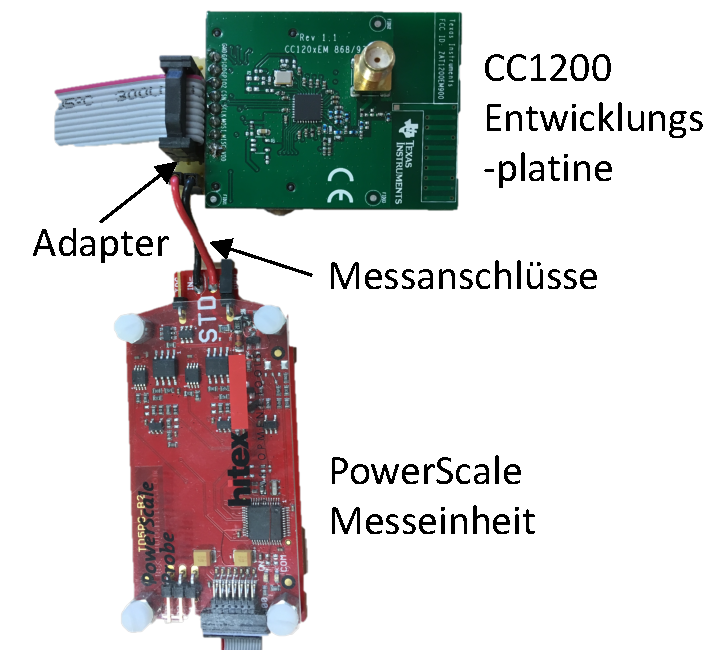
\includegraphics[width=0.4\linewidth]{gfx/Messdetail}} 
        \caption[Energiemessung]{Aufbau zur Energiemessung des CC1200 \glspl{transceiver}}\label{fig:mess}
\end{figure}

Zur Messung des Stroms in einem elektrischen System muss das Strommessgerät in den Stromkreislauf integriert werden. Ein Schaltbild des Messaufbaus ist in \autoref{fig:mess-schema} dargestellt. Um diese Integration des PowerScale-Systems zu ermöglichen, ist ein Adapter notwendig, der die Stromzufuhr des gls{cc1200} unterbricht und die Anschlusspunkte für das Messsystem bereitstellt. \autoref{fig:mess-detail} zeigt den Anschluss im Detail. Durch die Verbindungen zur Messeinheit wird die Stromzufuhr zum Funkchip wieder geschlossen.

Das Messprogramm auf dem Computer speichert den Verlauf der momentanen Leistungsaufnahme. Im Anschluss kann der für den jeweiligen Betriebsmodus relevante Zeitbereich ausgewählt werden und das Programm berechnet den Energieverbrauch durch Aufsummierung der gemessenen Leistungswerte für den markierten Zeitraum.

\section{Simulationen}\label{kap:grundlagen_sec:simulation}

Simulationen können dann eingesetzt werden, wenn ein System zu komplex für eine konkrete Berechnung ist oder ein Versuchsaufbau unverhältnismäßig aufwendig wäre. Nachdem ein System in einem Simulationsmodell implementiert ist, liegt der Vorteil darin, schnell einen Überblick über die Auswirkungen verschiedener Parametervariationen zu erhalten. Nachteilig ist, dass ein Simulationsmodell in der Regel nicht alle Aspekte des realen Systems berücksichtigt. Je detailreicher das Modell sein muss, desto größer ist der Aufwand der Implementierung. 

Im Bezug auf Netzwerke liegt der Vorteil von Simulationen darin, dass an vielen Stellen des Netzwerkes, \zB an Empfängern in einem Sensornetzwerk, derselbe Prozess stattfindet. Dieser Prozess muss nur einmal formal beschrieben sein und kann in der Simulation dann immer wieder zu entsprechender Zeit durchlaufen werden. Ebenso ist eine Übersicht aller in der Simulation enthaltenen Größen zu jedem Zeitpunkt möglich. Ein weiterer Vorteil besteht in der exakten Reproduzierbarkeit der Untersuchung.
\subsection{Ereignisorientierte Simulation}
Bei \acfp{des} werden die zu bearbeitenden Ereignisse $($engl. \emph{Events}$)$ in eine Liste, die so genannten \acf{fel}, eingeordnet und gemäß ihrer zeitlichen Abfolge bearbeitet. Ein einfaches Beispiel für eine \acs{des} ist der Kassiervorgang an der Supermarktkasse, wie in \autoref{fig:kasse} angedeutet. Eine entsprechende Simulation könnte ein Modell der einkaufenden Personen, ein Modell der Kasse und ein Modell der Warteschlange beinhalten. Wenn das Personenmodell die Menge an eingekauften Artikeln enthält, das Modell der Kasse die Bearbeitungszeit in Abhängigkeit der Artikelanzahl und das Modell der Schlange die Zahl der wartenden Personen verwaltet, läuft die Simulation wie folgt ab: Das Simulationsprogramm kann nach einer geeigneten Zufallsverteilung \gqq{Anstellen-\emph{Events}} erzeugen. Ist die Warteschlange leer, wird von dem Modell der Warteschlange direkt ein \gqq{Kassieren-\emph{Event}} erzeugt. Dadurch wird das Modell der Kasse aufgerufen, das die Bearbeitungszeit berechnet und ein \gqq{Verlassen-\emph{Event}} an entsprechender Stelle in die \acs{fel} einfügt.
Der Vorteil besteht darin, dass die Simulation nur die einzelnen \emph{Events} berechnen muss, die Zeit dazwischen wird nicht simuliert. Mit diesem Beispiel kann dann \zB die durchschnittliche Länge der Warteschlange in Abhängigkeit von der Menge der eingekauften Artikel berechnet werden.

\begin{figure}[bth]
        \myfloatalign
        {\includegraphics[width=0.6\linewidth]{gfx/kasse}} 
        \caption[Kasse]{angedeuteter Kassiervorgang als Beispiel für eine ereignisorientierte Simulation}\label{fig:kasse}
\end{figure}

Betrachtet man das genannte Beispiel aus einer abstrakten Sicht, so handelt es sich um ein System, bei dem eine Instanz, hier die Kasse, nach einer festgelegten Art eingehende Aufträge abarbeiten muss. Dieses Muster liegt auch den Vorgängen in Kommunikationsnetzen zugrunde, daher eignet sich eine \acl{des} besonders gut zur Unterschung von Netzwerken.

\subsection{OMNeT++}\label{kap:grundlagen_sec:omnet}
\gls{omnet} ist ein Simulationsframework für \acsp{des}, bei dem die Modellierung der einzelnen Komponenten in der Programmiersprache \gls{cpp} erfolgt. Wesentliche Aufgabe des Frameworks ist die Verwaltung der \acs{fel} und der Aufruf des Programmcodes der einzelnen Komponenten. \gls{omnet} bietet zusätzlich eine eigene Programmiersprache --- die \emph{NED}-Sprache --- an. Mit dieser können Gruppierung, Anordnung und Verbindungen der einzelnen Komponenten beschrieben werden.
Die wichtigsten Bestandteile von \acs{omnet} sind:
\begin{description}
\item[Module] Die einzelnen Komponenten der Simulation werden Module genannt. Mit der \gls{cpp}-Klasse \texttt{cModule} stellt das Framework eine Basisklasse zur Implementierung bereit. Während die Implementierung in \gls{cpp} erfolgt, wird die gegenseitige Beziehung zwischen verschiedenen Modulen in \emph{NED} beschrieben. Module können ineinander verschachtelt werden und besitzen Verbindungen zu anderen Modulen.

\item[Gates] Um \emph{Events} an andere Module zu senden, besitzen Module \emph{Gates}. Diese sind die eindeutigen Endpunkte einer Verbindung zwischen zwei Modulen. Schickt ein Modul ein \emph{Event} an ein \emph{Gate}, wird es genau dem Modul zugestellt, welches mittels der \emph{NED}-Sprache damit verknüpft ist. Module können mehrere \emph{Gates} besitzen. Außerdem können \emph{Events} direkt an ein \emph{Gate} eines anderen Moduls geschickt werden, ohne eine zuvor festgelegte Verbindung. Dies ist \zB für große Netzwerke mit variabler Anzahl an Teilnehmern sinnvoll. 

\item[Messages] \emph{Events} werden in \gls{omnet} \emph{Messages}, auf Deutsch \gqq{Nachrichten}, genannt. Im Zusammenhang mit Netzwerksimulationen ist anzumerken, dass dabei nicht zwangsläufig Nachrichten im Sinne des Netzwerkes gemeint sind, sondern dass es sich hierbei um jegliche Art von \emph{Event} in der Simulation handeln kann, \zB ein \emph{Timer-Event}.
\end{description}

\section{Hardware}\label{kap:grundlagen_sec:hardware}
In diesem Kapitel werden die Hardwarekomponenten vorgestellt, die zur prototypischen Implementierung des Systems verwendet werden. Die für die Funkkommunikation zentrale Komponente ist der CC1200 Funkchip von Texas Instruments. Für die Implementierung des Kanalzugriffprotokolls und zur Ansteuerung des Funkchips kommt der MSP430FR9596 Mikrocontroller von Texas Instruments zum Einsatz. Für beide Chips steht eine Entwicklungsplatine zur Verfügung.
\begin{figure}[bth]
        \myfloatalign
        \subfloat[MSP430 LaunchPad]
        {\label{fig:platinen-msp}%
        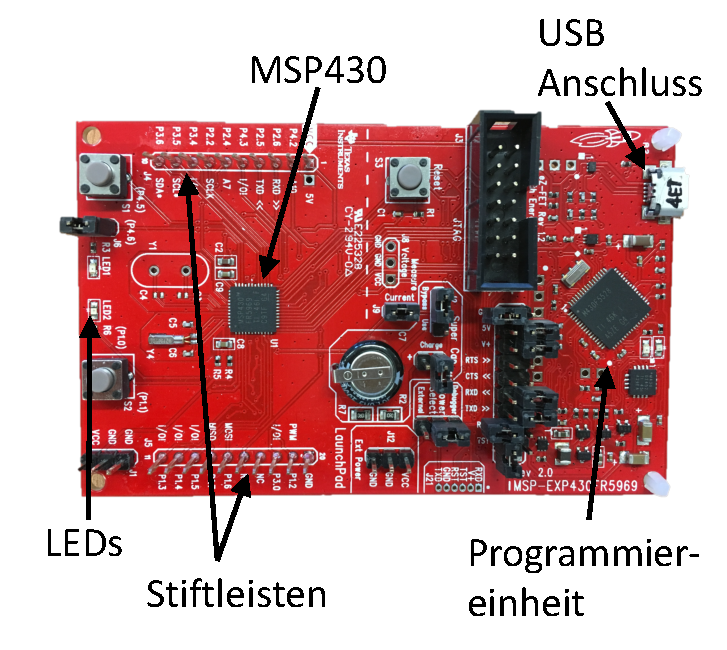
\includegraphics[width=0.5\linewidth]{gfx/MSP_Board}} 
        \subfloat[CC1200 EM]
        {\label{fig:platinen-cc1200}%
        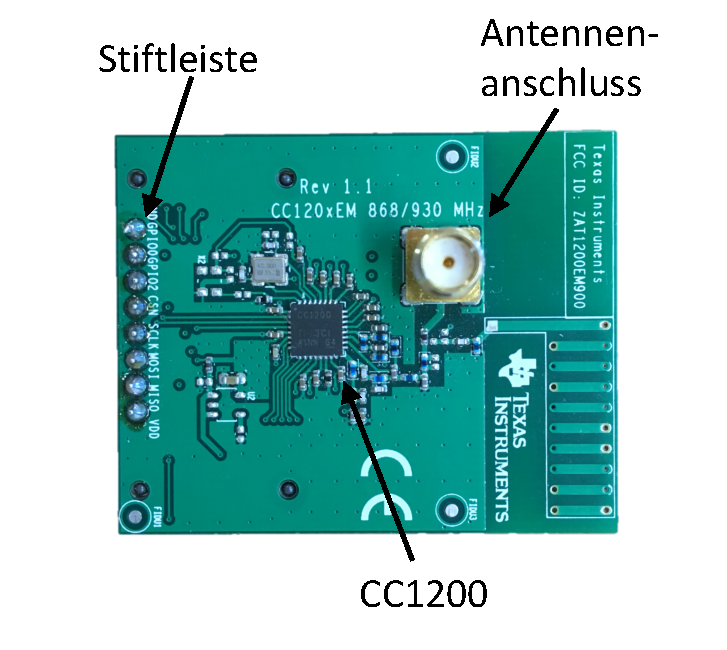
\includegraphics[width=0.5\linewidth]{gfx/CC1200_Board}} 
        \caption[Entwicklungsplatinen]{Entwicklungsplatinen für Mikrokontroller und \gls{transceiver} zur prototypischen Anwendungsimplementierung}\label{fig:platinen}
\end{figure}
Entwicklungsplatinen vereinfachen die Entwicklung von Anwendungen, indem sie die nötige Beschaltung der Chips mit zusätzlichen Bauelementen realisieren und wichtige Schnittstellen zur Verfügung stellen. \autoref{fig:platinen-msp} zeigt das MSP430 \emph{LaunchPad}. Dieses verfügt neben zwei \acsp{led}, zwei Tastern über Elektronik zur Programmierung des Mikrocontrollers per USB Verbindung. Daneben sind einige der \acs{gpio}-Pins zur einfachen Verdrahtung an Stiftleisten herausgeführt. In \autoref{fig:platinen-cc1200} ist die CC120x EM Platine zu sehen. Darauf ist der CC1200 Funkchip mit den entsprechenden externen Kondensatoren und Widerständen versehen, die für exakte Frequenzerzeugung notwendig sind. Weiterhin ist ein coaxialer Antennenanschluss vorhanden. An der Stiftleiste auf der linken Seite befinden sich die Signalleitungen zur Ansteuerung des Funkchips.

Die folgenden Abschnitte beschreiben die beiden Hardwarekomponenten im Detail und geben wichtige Hinweise für die Implementierung.

\subsection{MSP430}\label{kap:grundlagen_sec:msp430}
Mikrocontroller vereinen einen Prozessor (\acs{cpu}), Speicher und weitere Peripherie, wie Timer, acf{adc} und serielle Kommunikation in einem Chip. Die einzelnen Pins des Mikrocontrollers können zur Ansteuerung von Aktoren oder zum Auslesen von Sensoren genutzt werden. Die Pins werden als \acf{gpio}-Pins bezeichnet. Die Mikrocontroller der MSP430 Reihe sind darüber hinaus speziell für Anwendungen mit begrenzten Energieressourcen konzipiert. \autoref{tab:msp} zeigt die Hauptmerkmale des verwendeten Modells.

\begin{table}
    \myfloatalign
  \begin{tabularx}{0.7\textwidth}{Xll} \toprule
    %\tableheadline{Modus} & \tableheadline{Stromaufnahme} & \tableheadline{Leistungsaufnahme}\\ \midrule
    Modell & MSP430FR9596 \\
    Hersteller & Texas Instruments \\
    Betriebsspannung & 1,8V - 3,6V \\
    Architektur & 16 Bit \gls{risc} \\
    Taktrate & 32kHz - 24MHz \\
    Speicher & 64kB \acs{fram} \\
    \bottomrule
  \end{tabularx}
  \caption[MSP Merkmale]{Eigenschaften des MSP430 Mikrocontrollers \citep{MSPdata}}  \label{tab:msp}
\end{table} 

Die Programmierung erfolgt üblicherweise in der Programmiersprache \gls{c}. Für die Konfiguration und Ansteuerung der einzelnen Peripheriekomponenten sind spezielle Register im Speicher des Mikrocontrollers vorgesehen. Obwohl sie sich für das Programm wie normale Speicheradressen verhalten und auch so beschrieben oder gelesen werden können, steuern die Bits dieser Register das Verhalten der integrierten Peripherie. So bestimmt beispielsweise der Wert in einem \acs{gpio}-Register die Spannungspegel der Pins am entsprechenden Port. Andersherum kann aus Registern, die dem \acs{adc} zugeordnet sind, das Ergebnis der Analog-Digital Wandlung entnommen werden. Da auf Mikrocontrollern in vielen Fällen kein Betriebssystem läuft, das einzelne Programmstarts verwaltet, wird ein Programm für Mikrocontroller als Endlosschleife programmiert, wie in \autoref{lst:while} angedeutet.
\begin{lstlisting}[float=h,language=C,frame=tb,captionpos=b,caption={Strukturbeispiel eines Programms für Mikrocontroller},label=lst:while]
// Code, der zu Beginn einmal durchlaufen wird
// zB. Konfigurationen der Peripherie

while(1) {
	// hier erfolgt die Implementierung der Anwendung
}

// Programmende wird nie erreicht
\end{lstlisting}

Da die Entwicklung des Programms nicht auf dem Mikrocontroller selbst stattfindet, wird eine Software benötigt, die das \gls{c}-Programm für die Verwendung auf dem Chip kompiliert. Im Anschluss wird der Quellcode mit einem \emph{Programmer} auf den Chip übertragen. Auf dem \emph{LaunchPad} ist dieser, wie eingangs erwähnt, bereits vorhanden.

Für die Realisierung von Anwendungen mit geringer Leistungsaufnahme kann der MSP430 in sieben unterschiedliche Energiesparmodi versetzt werden, bei denen stufenweise einzelne Komponenten und Taktquellen abgeschaltet werden. Bei der 	Rückkehr aus den Modi 3.5 und 4.5 bleiben alle Pins des Controllers durch das Kontrollbit \texttt{LOCKLPM5} im \texttt{PM5CTL0} Register gesperrt, um zunächst alle Konfigurationen vorzunehmen und die Pins anschließend freizugeben. Dieser Zustand tritt auch nach jedem Systemstart ein. Um die Pins des MSP430 nutzen zu können, muss dieses Bit zu beginn des Programms auf Null gesetzt werden.

Eine weitere Besonderheit beim MSP430 ist, dass der \gls{watchdog}-\emph{Timer} standardmäßig aktiviert ist. Ein \gls{watchdog}-\emph{Timer} ist ein Zähler, der unabhängig von der \acs{cpu} hardwareseitig in einigen Mikrocontrollern integriert ist und bei Erreichen eines eingestellten Wertes einen Neustart des Systems auslöst, so er nicht regelmäßig vor seinem Ablauf durch die Software zurückgesetzt wird. Diese Technik dient dem automatischen Neustart des Controllers, für den Fall eines unerwarteten Fehlverhaltens. Es ist beim MSP430 daher darauf zu achten, den \gls{watchdog}-Timer entsprechend regelmäßig zurückzusetzen oder ganz zu deaktivieren.

Drei für die Programmierung des Funkchips und die Implementierung des Kanalzugriffverfahrens wichtige Komponenten sind die Interrupt-Behandlung, die Verwendung von \emph{Timern} und die \gls{gl:spi} Kommunikation.

\paragraph{Interrupts}
Um auf Ereignisse Ereignisse, wie das eintreffen eines Bytes über die serielle Schnittstelle, die Änderung des Spannungspegels an einem Pin oder den Ablauf eines \emph{Timers} reagieren zu können, kann der normale Programmablauf durch einen Interrupt unterbrochen werden. Tritt ein Interrupt ein, wird zunächst das zugehörige Interrupt /emph{Flag} zur Signalisierung gesetzt. Ist der jeweilige Interrupt softwareseitig aktiviert, beginnt der Mikrocontroller mit der Abarbeitung einer separaten Programmsequenz - der \acf{isr}. Die Startadresse dieses Programmabschnitts ist in der Interruptvektor Tabelle gespeichert. Der MSP430 verfügt über 26 verschiedene Interruptvektoren, die zum Großteil den Peripheriekomponenten zugeordnet sind. Einigen Komponenten sind auch zwei Vektoren zugeordnet. So können individuelle Behandlungsroutinen (\acsp{isr}) geschrieben werden, ohne erst die Quelle des Interrupts ermitteln zu müssen. Dies führt zu einer schnelleren Behandlung des Ereignisses. Ist die \acl{isr} abgearbeitet, wird mit dem normalen Programmablauf fortgefahren. 

Bei der Verwendung von Interrupts ist darauf zu achten, dass es nicht zu unkontrollierten Manipulationen von gemeinsam genutzten Daten kommt. Durchläuft das Hauptprogramm \zB ein Array, in dem die Daten der letzten seriellen Übertragung gespeichert sind, muss sicher gestellt werden, dass diese Daten bis zum Ende des Durchlaufs nicht von einer \acs{isr} überschrieben werden.

\paragraph{Timer}
Der Grundbaustein eines \emph{Timers} ist ein Zählregister, dessen Wert in definierten Abständen inkrementiert wird. Diese Abstände hängen mit dem Systemtakt zusammen. Die Taktrate des Zählers lässt sich über Vorteiler bezogen auf die Systemtaktrate einstellen. Durch diese Einstellung wird die minimal zu messende Zeit des \emph{Timers} festgelegt. Die Größe des Zählregisters bestimmt die Auflösung des \emph{Timers}, also die Anzahl von Schritten bis zum Erreichen des Höchstwertes und damit zum Ablauf \emph{Timers}. Die Funktionsweise ist in \autoref{fig:timer} für eine Auflösung von vier Bit, also acht Zählwerten, verdeutlicht. Die Auflösung beim MSP430 beträgt 16 Bit.
\begin{figure}[bth]
        \myfloatalign
        {\includegraphics[width=\linewidth]{gfx/Timer}} 
        \caption[Timer]{Funktionsweise eines 4-Bit \emph{Timers}. Der rotmarkierte Wert kennzeichnet den eingestellten Vergleichswert.}\label{fig:timer}
\end{figure}
Da die Einstellung der Taktrate $f_\textrm{Timer}$ nur in bestimmten Schritten möglich ist, bietet der MSP430 zusätzlich die Möglichkeit, einen Interrupt auszulösen, wenn ein definierter Vergleichswert erreicht wird, in \autoref{fig:timer} in rot markiert. Dieser Wert kann über ein Register eingestellt werden und erlaubt so ein sehr feine Einstellung des Interruptzeitpunkts.

\paragraph{SPI}
Das \acf{spi} des Mikrocontroller bietet die Möglichkeit eine synchrone serielle Buskommunikation mit Peripheriegeräten, wie \zB dem CC1200 Funkchip, herzustellen. Die Kommunikation wir dabei stets von einem Gerät initialisiert, dem \emph{Master}. Die angeschlossenen Geräte werden als \emph{Slaves} bezeichnet. Dazu werden drei gemeinsame Signalleitungen benötigt und zusätzlich eine Leitung pro \emph{Slave}:
\begin{enumerate}
\item \gls{gl:mosi}
\item \gls{gl:miso}
\item \gls{gl:scl}
\item \gls{gl:cs}
\end{enumerate}

Zu Beginn der Kommunikation muss der \emph{Master} die beteiligten Kommunikationspartner aktivieren, dies geschieht über die \gls{gl:cs}, engl. \acl{cs}.
Anschließend erzeugt der \emph{Master} auf der \gls{gl:scl} regelmäßige Signalflanken, engl. \acl{scl}. Mit dieser Frequenz wird dann der Pegel der \gls{gl:mosi} entsprechend der zu übertragen Bits auf Null oder Eins geändert, sodass der \emph{Slave} diese bei jeder Taktflanke abtasten kann, engl. \acl{mosi}. Gleichzeitig kann der \emph{Slave} über die \gls{gl:miso} Daten an den \emph{Master} in analoger Weise senden, engl. \acl{miso}.
Der MSP430 realisiert diese Bussystem in einer Hardwareeinheit zur seriellen Kommunikation. Nach entsprechender Konfiguration, kann ein zu sendendes Byte in dafür vorgesehenes Register geschrieben werden. Der Controller startet dann automatisch den Kommunikationsvorgang. Die übertragenen Daten des \emph{Slaves} werden ebenfalls in einem Register abgelegt und können ausgelesen werden. Nach vollständiger Übertragung kann ein Interrupt ausgelöst werden. Ein Mitschnitt der \gls{gl:spi} Kommunikation zwischen MSP430 und dem CC1200 Funkchip ist in \autoref{fig:spi} zu sehen.

\subsection{CC1200 Funkchip}\label{kap:grundlagen_sec:cc1200}
Der CC1200 Funkchip von Texas Instruments ist ein Transceiver für den Sub-GHz Bereich mit umfassenden Konfigurationsmöglichkeiten zur Sendefrequenz, Moduation (vgl. \autoref{kap:grundlagen_sec:modulation}), zur Paketverarbeitung und Kanalprüfung. Die wesentlichen Merkmale sind in \autoref{tab:cc1200} aufgelistet. Einen besonders sparsamen Betrieb erreicht der CC1200 durch den sogenannten \emph{Sniff}-Modus. \autoref{fig:sniff} veranschaulicht die Vorteile gegenüber dem normalen Empfangsmodus. Der \gls{transceiver} fügt vor den Nutzdaten eine Präambel und ein Synchronisationsbyte ein, um den Beginn der Nachricht zu markieren und die Empfangselektronik kalibrieren zu können. Der CC1200 ist in der Lage den Beginn einer Nachricht nach ein vier Präambel-Bits zu detektieren. Des Weiteren benötigt der Chip nur ca. $0,6ms$ um vom Ruhemodus in den Empfangsmodus zu wechseln \citep{CC1200data}. Diese Eigenschaften erlauben es im \emph{Sniff}-Modus in regelmäßigen Abständen kurz in den Empfangsmodus (RX) zu schalten, während der Chip zum größten Teil im energiesparenden Ruhemodus verbleibt. Dazu muss die Präambellänge deutlich erhöht werden, um kein Paket zu verpassen, wie in \autoref{fig:sniff2} zu erkennen ist. Sie muss so groß sein, dass im dargestellten ungünstigsten Fall - das Paket beginnt genau nach dem der Chip gerade in den Ruhemodus gewechsel ist - noch mindestens vier Präambel-Bytes beim nächsten Wechsel zu RX detektiert werden können. Es ist noch anzumerken, dass dieses Verfahren nur für den Empfang von Paketen vorgesehen ist. Zum Zweck der Kanalüberprüfung ist der kontinuierliche RX-Modus nötig.

\begin{table}
    \myfloatalign
  \begin{tabularx}{\textwidth}{Xll} \toprule
    %\tableheadline{Modus} & \tableheadline{Stromaufnahme} & \tableheadline{Leistungsaufnahme}\\ \midrule
    Modell & CC1200 \\
    Hersteller & Texas Instruments \\
    Betriebsspannung & 3,3V \\
    primäre Frequenzen & 169MHz, 433MHz, 868MHz, 915MHz \\
    maximale Sendeleistung & 16dBm \\
    Empfindlichkeit & -109dBm bei 50kBits/s \\
    maximale Datenrate & 1,25MBits/s  \\
    Sende-/Empfangsspeicher & je 128 Byte  \\
    \bottomrule
  \end{tabularx}
  \caption[CC1200 Merkmale]{Eigenschaften des CC1200 Funkchips \citep{MSPdata}}  \label{tab:cc1200}
\end{table}

\begin{figure}[bth]
        \myfloatalign
        \subfloat[Normaler Empfangsmodus]
        {\label{fig:sniff1}%
        \includegraphics[width=\linewidth]{gfx/Sniff1}} \\
        \subfloat[Sniff Modus]
        {\label{fig:sniff2}%
        \includegraphics[width=\linewidth]{gfx/Sniff2}} 
        \caption[CC1200 Sniffmode]{Auszug aus dem CC1200 \emph{User's Guide} zur Veranschauichung des energiespareden \emph{Sniff}-Modus \citep{CC1200guide}}\label{fig:sniff}
\end{figure}

Die Ansteuerung des CC1200 Funkchips erfolgt über \gls{gl:spi}. Der Informationsaustausch zwischen Mikrocontroller und CC1200 lässt sich dazu in drei Rubriken einteilen:
\begin{enumerate}
\item Schreiben bzw. Lesen der insgesamt 209 Konfigurationsregister zur Einstellung der Sendefrequenz, Modulationsart, Paketlänge, etc.
\item Sende von Kommandos, den so genannten \emph{Strobes}, um die Funkchip in den gewünschten Modus zu versetzen.
\item Austausch von Sende- und Empfangsdaten.
\end{enumerate}

Die Art der Informationsübertragung wird durch das erste Byte bestimmt, welches der Mikrocontroller an den Funkchip sendet. Letzterer erwartet dann weitere Informationen in Form von Bytes in einem festgelegten Muster. Wird durch das erste Byte signalisiert, dass der Chip seinerseits Daten über den Bus senden soll, gilt dies analog. Für den Fall, dass keine Daten vom Chip angefordert werden, sendet dieser bei jeder Übertagung ein Statusbyte an den Mikrocontroller, aus dem der aktuelle Modus und etwaige Fehlermeldungen entnommen werden können. Diese individuellen Übertragungsmuster erfordern, dass die \gls{gl:cs} während des ersten Bytes und allen evtl. folgenden Bytes kontinuierlich durch den Mikrocontroller auf Null-Pegel gehalten wird. Dies ist bei Konfiguration des MSP430 zur automatischen \gls{gl:spi} Steuerung (vgl. \autoref{kap:grundlagen_sec:msp430}) nicht gegeben, da die \gls{gl:cs} dabei nach jedem Byte wieder deaktiviert wird. Um die Übertragung nicht abzubrechen, muss der Pin für die \gls{gl:cs} separat durch die Software angesteuert werden. Beispielhaft ist in \autoref{fig:spi} der Schreibvorgang in ein Konfigurationsregister des CC1200 zu sehen, dass sich im erweiterten Adressraum befindet. In diesem Fall signalisiert das erste Byte den  lediglich, dass es sich um einen Zugriff auf den erweiterten Adressraum handelt. Der Funkchip erwartet dann die Adresse im zweiten übertragenen Byte und schließlich den Wert, der an diese Adresse geschrieben werden soll.


\begin{figure}[bth]
        \myfloatalign
        {\includegraphics[width=\linewidth]{gfx/SPI}} 
        \caption[SPI]{Mitschnitt der SPI-Kommunikation zwischen MS430 und CC1200. Zu sehen ist der Schreibvorgang eines Konfigurationsregisters des CC1200 im erweiterten Adressraum.}\label{fig:spi}
\end{figure}

\section{Entwicklungssoftware}\label{kap:grundlagen_sec:software}

Neben der bereits in \autoref{kap:grundlagen_sec:omnet} beschriebenen Simulationsumgebung \gls{omnet} und dem in \autoref{kap:grundlagen_sec:energiemessung} vorgestellten \emph{PowerScale} System sind noch weitere Entwicklungs- und Diagnosewerkzeuge für diese Arbeit notwendig. Deren Aufgaben im Rahmen dieser Arbeit werden hier aufgeführt.

\begin{description}
\item[Code Composer Studio] Eine Entwicklungsumgebung zur Programmierung des MSP430 Mikrocontrollers. Neben der Verwaltung der einzelnen Quellcodedateien und der in \autoref{kap:grundlagen_sec:msp430} genannten Übersetzung des \gls{c}-Codes in Maschinenbefehle, bietet diese Software die Möglichkeit zum \emph{Debugging}, auf Deutsch \gqq{Fehlersuche}. Dabei kann der auf den Mikrocontroller geladenen Programmcode schrittweise ausgeführt werden. Außerdem können die Registerwerte und Variablen ausgelesen werden. Die Möglichkeit des \emph{Debuggings} muss von der Hardware unterstützt werde. Das \emph{LaunchPad} bietet diese Möglichkeit.

\item[RF Studio / Packet Sniffer] Zwei Softwarewerkzeuge die über eine Hardwareschnittsstelle --- denm \emph{CC12xx Debugger} --- die Register des CC1200 Funkchips direkt schreiben und auslesen können. Zum einen kann der Funkchip so auch ohne Mikrocontroller konfiguriert und in Betrieb genommen werden, zum anderen ist es möglich, empfangenen Daten auf dem Computer anzeigen zu lassen und einige Verarbeitungsinformationen des CC1200 auszulesen. Dazu gehören die Empfangsqualität, das Ergebnis der Bitfehlerprüfung sowie der Zeitstempel von empfangenen Nachrichten.

\item[hterm] Ein Terminalprogramm zur byteweisen seriellen Datenübertragung. Dieses wird benutzt, um Informationen mit dem Mikrocontroller auszutauschen. Dieser Informationsaustausch bezieht sich nicht auf die Programmierung des Controllers sondern auf den Austausch von Daten aus dem laufenden Programm heraus. Dabei besteht die Möglichkeit, die Daten sowohl in Textform, als auch in binärer oder hexadezimaler Darstellung einzugeben und anzeigen zu lassen. 
\end{description}
%*****************************************
%*****************************************
%*****************************************
%*****************************************
%*****************************************




